\documentclass[]{article}
\usepackage[T1]{fontenc}
\usepackage{lmodern}
\usepackage{amssymb,amsmath}
\usepackage{ifxetex,ifluatex}
\usepackage{fixltx2e} % provides \textsubscript
% use upquote if available, for straight quotes in verbatim environments
\IfFileExists{upquote.sty}{\usepackage{upquote}}{}
\ifnum 0\ifxetex 1\fi\ifluatex 1\fi=0 % if pdftex
  \usepackage[utf8]{inputenc}
\else % if luatex or xelatex
  \ifxetex
    \usepackage{mathspec}
    \usepackage{xltxtra,xunicode}
  \else
    \usepackage{fontspec}
  \fi
  \defaultfontfeatures{Mapping=tex-text,Scale=MatchLowercase}
  \newcommand{\euro}{€}
\fi
% use microtype if available
\IfFileExists{microtype.sty}{\usepackage{microtype}}{}
\usepackage[margin=1in]{geometry}
\usepackage{color}
\usepackage{fancyvrb}
\newcommand{\VerbBar}{|}
\newcommand{\VERB}{\Verb[commandchars=\\\{\}]}
\DefineVerbatimEnvironment{Highlighting}{Verbatim}{commandchars=\\\{\}}
% Add ',fontsize=\small' for more characters per line
\usepackage{framed}
\definecolor{shadecolor}{RGB}{248,248,248}
\newenvironment{Shaded}{\begin{snugshade}}{\end{snugshade}}
\newcommand{\KeywordTok}[1]{\textcolor[rgb]{0.13,0.29,0.53}{\textbf{{#1}}}}
\newcommand{\DataTypeTok}[1]{\textcolor[rgb]{0.13,0.29,0.53}{{#1}}}
\newcommand{\DecValTok}[1]{\textcolor[rgb]{0.00,0.00,0.81}{{#1}}}
\newcommand{\BaseNTok}[1]{\textcolor[rgb]{0.00,0.00,0.81}{{#1}}}
\newcommand{\FloatTok}[1]{\textcolor[rgb]{0.00,0.00,0.81}{{#1}}}
\newcommand{\CharTok}[1]{\textcolor[rgb]{0.31,0.60,0.02}{{#1}}}
\newcommand{\StringTok}[1]{\textcolor[rgb]{0.31,0.60,0.02}{{#1}}}
\newcommand{\CommentTok}[1]{\textcolor[rgb]{0.56,0.35,0.01}{\textit{{#1}}}}
\newcommand{\OtherTok}[1]{\textcolor[rgb]{0.56,0.35,0.01}{{#1}}}
\newcommand{\AlertTok}[1]{\textcolor[rgb]{0.94,0.16,0.16}{{#1}}}
\newcommand{\FunctionTok}[1]{\textcolor[rgb]{0.00,0.00,0.00}{{#1}}}
\newcommand{\RegionMarkerTok}[1]{{#1}}
\newcommand{\ErrorTok}[1]{\textbf{{#1}}}
\newcommand{\NormalTok}[1]{{#1}}
\usepackage{longtable,booktabs}
\usepackage{graphicx}
% Redefine \includegraphics so that, unless explicit options are
% given, the image width will not exceed the width of the page.
% Images get their normal width if they fit onto the page, but
% are scaled down if they would overflow the margins.
\makeatletter
\def\ScaleIfNeeded{%
  \ifdim\Gin@nat@width>\linewidth
    \linewidth
  \else
    \Gin@nat@width
  \fi
}
\makeatother
\let\Oldincludegraphics\includegraphics
{%
 \catcode`\@=11\relax%
 \gdef\includegraphics{\@ifnextchar[{\Oldincludegraphics}{\Oldincludegraphics[width=\ScaleIfNeeded]}}%
}%
\ifxetex
  \usepackage[setpagesize=false, % page size defined by xetex
              unicode=false, % unicode breaks when used with xetex
              xetex]{hyperref}
\else
  \usepackage[unicode=true]{hyperref}
\fi
\hypersetup{breaklinks=true,
            bookmarks=true,
            pdfauthor={Carl P. Lipo, Rene Horneman, Terry L. Hunt, Vincent Bonhomme},
            pdftitle={Rapa Nui Mataa Morphometric Analyses},
            colorlinks=true,
            citecolor=blue,
            urlcolor=blue,
            linkcolor=magenta,
            pdfborder={0 0 0}}
\urlstyle{same}  % don't use monospace font for urls
\setlength{\parindent}{0pt}
\setlength{\parskip}{6pt plus 2pt minus 1pt}
\setlength{\emergencystretch}{3em}  % prevent overfull lines
\setcounter{secnumdepth}{0}

%%% Change title format to be more compact
\usepackage{titling}
\setlength{\droptitle}{-2em}
  \title{Rapa Nui Mataa Morphometric Analyses}
  \pretitle{\vspace{\droptitle}\centering\huge}
  \posttitle{\par}
  \author{Carl P. Lipo, Rene Horneman, Terry L. Hunt, Vincent Bonhomme}
  \preauthor{\centering\large\emph}
  \postauthor{\par}
  \predate{\centering\large\emph}
  \postdate{\par}
  \date{7 September 2014}




\begin{document}

\maketitle


\section{Introduction}\label{introduction}

Rapa Nui (Easter Island, Chile) is a tiny island located in a remote
corner of Eastern Polynesia, more than 2000 km from the nearest
inhabited body of land (Figure 1). The island was first colonized by
Polynesians who sailed from central East Polynesia in voyaging canoes
during the 13th century AD (Hunt \& Lipo 2006; Wilmshurst \emph{et al.}
2011). Depsite the island's diminuitive size, remoteness, and limited
natural resources, the archaeological record of Rapa Nui is well-known
for its nearly 1000 multi-ton statues known as \emph{moai} that once sat
atop massive stone platforms known as \emph{ahu} (Hunt \& Lipo 2011a).

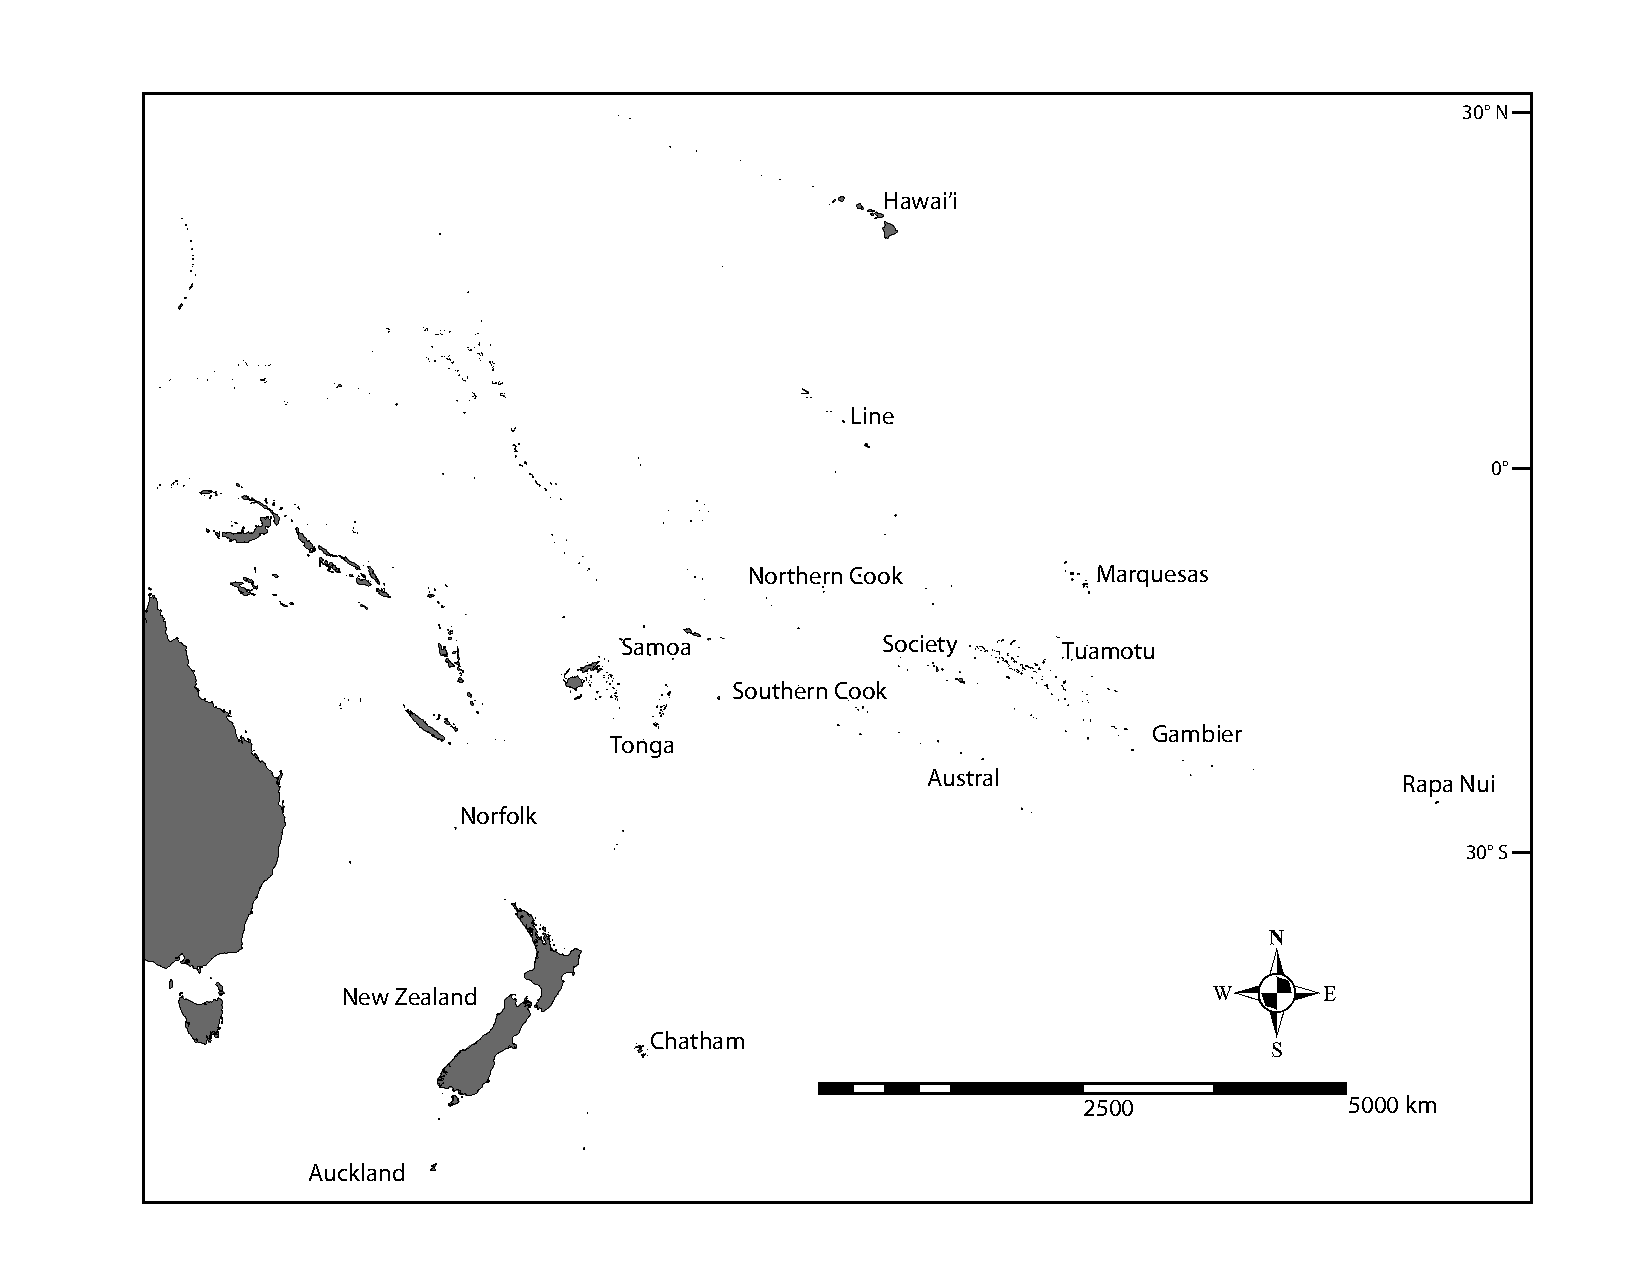
\includegraphics{../Figures/Figure1.pdf}

The dramatic prehistoric investment in monumental architecture stand in
marked contrast to the Rapa Nui's environment and historically observed
population levels. Even at the first point of European contact, the tiny
island was largely devoid of trees and population sizes were just about
3000 individuals (Hunt \& Lipo 2011a, p.~XXX). While earlier researchers
(e.g., Heyerdahl \& Ferdon 1965; Heyerdahl 1989) believed the depleted
and depauperate state of the island was due to conflict between
Polynesians and elite from South America, more recent reseachers have
interepreted the contrast between the spectacular nature of the
archaeological record and the sparse enviornment of the island as the
outcome of a prehistoric environmental catastrophe (Bahn \& Flenley
1992; Flenley \& Bahn 2003). These researchers argue that based largely
on oral traditions, that prehistoric populations grew in numbers until
resource use exceeded the carrying capacity and the island underwent
catastropic demographic collapse. This account has been popularlized as
the ``collapse'' scenario (\emph{sensu} Diamond 1995; 2005).

New research, however, has challenged this notion with empirical
evidence generated from the archaeological record that the Rapanui
flourished on the island until AD 1722 when Europeans brought diseases
and other social disruptions (Hunt 2007; Hunt \& Lipo 2007; Hunt \& Lipo
2009a; Hunt \& Lipo 2009b; Hunt \& Lipo 2011a; Hunt \& Lipo 2011b; Lipo
\& Hunt 2009; Mulrooney \emph{et al.} 2009; Mulrooney 2012; Rainbird
2002). Investigations on Rapa Nui's settelement patterns demonstrates
that the island's inhabitants lived in a dispersed pattern in a low
density fashion (Hunt \& Lipo 2011a; Morrison 2012). In addition,
studies show that subsistence was largely based on extensive but
marginally productive lithic mulch gardens to boost the nutrient-poor
soil to a level that sustained sweet potato cultivation (Bork \emph{et
al.} 2004; Ladefoged \emph{et al.} 2005; Ladefoged \emph{et al.} 2010;
Ladefoged \emph{et al.} 2013; Mieth \emph{et al.} 2010; Stevenson \&
Haoa 2002; Stevenson \emph{et al.} 2006). Finally, demise of the once
extensive palm tree forest appears to have had little to do with statue
construction or changes in carry capacity (Hunt \& Lipo 2011a; Lipo
\emph{et al.} 2013).

One of the claims that persists that is thought to support the
``collapse'' scenario is the idea that prehistoric Rapa Nui populations
experienced intense warfare during late prehistory when resources became
increasingly scarce (Bahn \& Flenley 1992; Diamond 1995, Diamond (2005);
Flenley \& Bahn 2003). Oral traditions are known that attribute the
toppling of stone statues to intertribal prehistorc warfare (Bahn \&
Flenley 1992). But the existence of fallen statues alone does not
necessarily imply warfare since other natural explanations are more
likely (Edwards \emph{et al.} 1996). Indeed, the existing evidence
points to the toppling of statues as as series of post-contact historic
events rather than prehistory (Hunt \& Lipo 2011a). Most significantly,
examples of defensive structures are entirely lacking in the island's
archaeological record (Hunt \& Lipo 2011a; Lipo \& Hunt 2014). Overall,
much of the evidence for prehistoric warfare among the inhabitants of
Rapa Nui comes from oral traditions recorded in the 20th century (e.g.,
Routledge 1919). The oral traditions, however, have an unknown relation
to prehistory. Metraux {[}\href{mailto:-@1940}{-@1940}:aa, p.~XXX{]},
for example, argues that most of the traditions are likely recent and
thus likely do not reflect prehistoric events. Given the unknown origins
of oral traditions, we must rely upon direct archaeological evidence for
warfare.

The one example of empirical evidence used to support arguments about
prehistoric warfare on Rapa Nui is the presence of \emph{mata'a}, flaked
obsidian stemmed tools. \emph{Mata'a} are a class of hafted flaked
obsidian artifacts that are found commonly on Rapa Nui. As relatively
simple stemmed obsidian tools with wide blades, their form is similar to
artifacts known as \emph{mata} found on other Polynesian islands such
the basalt artifacts found on New Zealand, Pitcairn and the Chatham
Islands (Balfour 1917; Metraux 1957: 232; Skinner 1958) as well as New
Britain, Papua New Guinea (e.g., Araho 1997; Specht \emph{et al.} 1988;
Torrence, Swadling, \& Ambrose\emph{et al.} 2009; Torrence, Swadling, \&
Kononenko\emph{et al.} 2009; Torrence \emph{et al.} 2013).

In the current analysis, we seek to explore whether there exists
variability in the shape of \emph{mata'a} that sheds provides
information about the fucntional environment in which these artifacts
interacted. Using a large image database of `r numberOfMataa'
\emph{mata'a} from Rapa Nu, we conduct quantitative morphometric
analyses to further investigate whether specific tool classes might be
identifiable in the range of shapes in which these artifacts are found.
Morphometric analyses enable on to explore shape as a continuous
property of objects rather than requiring us treat shape as nominal
categories. In this way we can use principal components analyses to see
of particular kinds of shapes map to particular locations, environments
or source material. In addition, we can examine the relative patterns
\emph{mata'a} shape variability and to look for areas of shape that are
constrained versus those that were more free to vary. Overall, our
results conclude that mata'a were only functionally constrained in terms
of the haft and had signficant variation on the distal end and blade.
These results continue to support the alternative hypotheses that these
artifacts were not used as weapons. The degree of similarity, however,
of the haft portion of \emph{mata'a} and the low degree of constraint in
the blade poses an intriguing puzzle: we have yet to identify the
role(s) that these objects played in Rapa Nui subsistence and
settlement.

\section{Approach}\label{approach}

\emph{Mata'a} have been noted since the earliest European visitors
described the island. Members of Cook's expedition to the island
commented that the islanders ``had lances or spears made of thin
ill-shaped sticks, and pointed with a sharp triangular piece of black
glassy lava'' (Saher 1990: 35). \emph{Mata'a} are often assumed to be
``spears'' largely because of their resemblance to European varieties
rather than any direct observation of their use. Scars noted by early
European observers are also believed to have been inflicted by
\emph{mata'a} though there is no clear evidence that their use was
lethal. For example, in his voyage to Rapa Nui in 1770, Captain Don
Felipe González (Haedo \& Roggeveen 1908: (13):99) remarked that ``they
{[}Rapanui{]} possess no arms, and although in some we observed sundry
wounds on the body, which we thought to have been inflicted by cutting
instruments of iron or steel, we found that they proceeded from stones,
which are their only {[}weapons of{]} defence and offence, and as most
of these are sharp edged they produce the injury referred to.''

Even if we had direct observations of these objects being used in
``spear-like'' fashion, the unavoidable tendency for these European
observers to interpret what they saw through their own preconceptions
requires us examine the physical evidence available on mata'a. In this
way we can learn not only the range of interactions that the objects had
with the environment but also determine if there is variablity in their
use through time or over space.

On the surface landscape of Rapa Nui, \emph{mata'a} are one of the most
numerous shaped artifact classes. Overall, \emph{mata'a} vary greatly in
size and shape, but average 6-10 cm in width and length.
Technologically, they are formed from unifacial flakes derived trough
hard hammer percussion on obsidian cores quarried from one of the
island's obsidian sources. Most of the shaping of the \emph{mata'a}
occurs during the creation of a stem that presumably serves as a haft.
The stem is formed from one of the lateral margins of the original flake
where blade constitutes the remaining distal and opposite lateral
margins. \emph{Mata'a} stems and shoulders are formed by unifacial
flaking and are generally lenticular in cross section. Overall, the
blade shape is dominated by the shape of the parent flake though some
shaping through secondary flaking is sometimes evident. Often, large
areas of cortex still cover much of one face.

In exploring the the way in which \emph{mata'a} forms vary, researchers
have noted that there is a great diversity of shape and this feature has
remained one particularly puzzling aspect of
\emph{mata\texttt{a* {[}@Mulloy:1961aa{]}. *Mata}a} shapes are highly
inconsistent and vary from rounded to subangluar to angular to complex.
Early researchers assigned mata`a shape variation to what they conceived
as ethnographic categories based on Rapanui words (i.e., Routledge
1919). Later attempts to construct systematic classifications have also
focused on identifying types based on characterizations of overall
shape. None of these classification efforts produced useful categories.

Mulloy (1961: 151), for example, argued that ``no significant clustering
or correlations could be extracted\ldots{}. the material represents a
continuous range of variation without objective natural order, and that
the only classification possible must involve the subjective selection
of ideal types from infinite series of possibilities, and the arbitrary
reference of intermediate for to one or another of these.'' Mulloy
concluded manufacturing procedures dictated shapes and differences in
overall shape of mata'a were best explained by chance.

The overall shape of an object is rarely a useful dimension for
problem-oriented classification (Dunnell 1986). The forms of objects are
limited by technological constraints of the material, performance
aspects that depend upon the range of environments in which the object
is used, and simple idiosyncratic variability related to the
manufacturer and the process of production. In the case of \emph{mata'a}
much of the variability in the overall blade shape can be explained by
the contingent results involved in the stages of manufacture (Bollt
\emph{et al.} 2006). The difference in shapes, therefore, may have
structured functional variation related to the range and kinds of
activities for which the tool was primarily used. Studies of use-wear
found on \emph{mata'a} point to the tool being used primarily for
scraping and cutting or some combination (Church \& Rigney 1994; Church
\& Ellis 1996).

A recent study of \emph{mata'a} shape using stylistic classes and
deterministic frequency seriation as a means for examining how class
frequencies changed over space and through time showed remarkably
continuous change (Lipo \emph{et al.} 2010). The seriation results
suggest that the source of variability in \emph{mata'a} form is largely
being inherited through the social learning of manufacturing techniques
between indivdiuals. The evidence also indicates that variability in the
form of \emph{mata'a} is not related to how the \emph{mata'a} performed
in its use environment(s). Overall, our growing understanding of
\emph{mata'a} variability continues to support their form being related
to ceremonial or cultivation activities and not as weapons invovled in
warfare (Bollt \emph{et al.} 2006; Lipo \emph{et al.} 2010).

In our analysis here, we focus on \emph{mata'a} variability in the blade
portion of the mata'a relative to the stem. We assume that as hafted
objects the point at the center of the stem where it meets the blade can
be held constant for comparisons of shape. We then assume that due to
performance the functional aspects of the tool will result in shape
variability that is more constrained than the non-functional or
stylistic attributes (Lipo \emph{et al.} 2012). The constraints are the
result of natural selection that serves to sort shape variability in
proportion to the benefits/drawbacks to performance. Based on this
notion, we hypothesise that:

\begin{itemize}
\item
  If \emph{mata'a} are weapons, the distal end of the artifact will be
  constrained. However, if \emph{mata'a} are not weapons, other areas of
  the tool will show greater constraint consistent with alternate
  functions.
\item
  If \emph{mata'a} are weapons, the distal end of the artifact will show
  a tendency towards a pointed spear-like shape that will penetrate
  either enemies or prey. If \emph{mata'a} are not weapons, there will
  be no such constrictive tendency at the distal end of the tool.
\item
  If there was inter-tribal warfare, \emph{mata'a} from distinct areas
  may show stylistic traits of distinct groups. If natives were not
  divided into warring groups, distinct stylistic traits may or may not
  be apparent.
\end{itemize}

\section{Methods and Data}\label{methods-and-data}

In order to test these hypotheses, we used morphometric outline
analysis. Morphometrics is the quantitative analysis of form in terms of
shape and size (Bookstein 1982; Bookstein \emph{et al.} 1985; Bookstein
1997; Cardillo 2010; Kendall 1989; Rohlf 1990). It has advantages over
traditional studies of shape that treat shape as a nominal character
(e.g., ``triangular'', ``square'', ``round''). Even classifications that
break shape into a series of dimensionally constructed classes reduce
variability into modal categories. Morphometrics avoid the problem of
nominal shape by analyzing the form of objects as a series of metric
measurements that characterize the relative positions of series of
landmarks or comprise the outline. Analysies of form variability can be
conducted in two and three dimensions (Kendall 1989). With techniques
available for standardizing scale and rotation, morphometric
measurements directly compare outlines of artifacts and generate data on
the variations between artifacts. Consequently, one major feature of
morphometrics is its ready ability to statistically test hypotheses
about the factors that affect shape.

Measurements for morphometrics can be generated in a number of ways.
With roots in biology, the earliest form of morphometrics focused on
identifying the location specific landmarks (e.g., Thompson 1917). A
landmark approach requires defining features of interest that are to be
examined as to how they relate to each other. In the case of artifacts
such as \emph{mata'a} there are few consistent landmarks to hold
constant other than perhaps the distal and proximal end. One can also
one can conduct an analysis of what is known as ``semi-landmarks,'' a
fixed number of regularly positioned points around the outline of an
object (Bookstein 1997; Gunz \& Mitteroecker 2013). Both approaches to
measuring shape make use of the relative positions between all points
(Bookstein 1991; 1997).

In our morphometric analyses we make use of Momocs
(\url{http://CRAN.R-project.org/package=Momocs}), an R package (R Core
Team 2014) developed by Bonhomme (2012; Bonhomme \emph{et al.} 2014).
Momocs builds upon techniques developed by Claude (2008) and reviewed by
Bowman (2009). Bonhomme incorporated functions from Claude's work into
an integrated framework and a standalone R package. The package's
vignette \emph{A Graphical Introduction to Momocs and Outline Analysis
Using R} (Bonhomme 2012) provides an extensive description of the
functions of the package.

Table 1: \emph{Mata'a} included in analyses by collection.

\begin{longtable}[c]{@{}lrrrrr@{}}
\toprule\addlinespace
& Ahu Tautira & Orito & Orongo & Rano Kau & Unknown
\\\addlinespace
\midrule\endhead
Bishop & 0 & 0 & 0 & 0 & 291
\\\addlinespace
Engert & 25 & 31 & 29 & 33 & 0
\\\addlinespace
Heyerdahl & 0 & 0 & 0 & 0 & 8
\\\addlinespace
\bottomrule
\end{longtable}

Table 2: \emph{Mata'a} included in analyses by location.

\begin{longtable}[c]{@{}lrrrrr@{}}
\toprule\addlinespace
& Ahu Tautira & Orito & Orongo & Rano Kau & Unknown
\\\addlinespace
\midrule\endhead
Motu Iti & 0 & 0 & 0 & 0 & 5
\\\addlinespace
Orito & 0 & 0 & 0 & 0 & 279
\\\addlinespace
Rano Kau 1 & 0 & 0 & 0 & 0 & 7
\\\addlinespace
Unknown & 25 & 31 & 29 & 33 & 8
\\\addlinespace
\bottomrule
\end{longtable}

For our analyses of Rapa Nui \emph{mata'a}, our assemblage consisted of
planview photographs of (N=`r numberOfMataa') artifacts from two museum
collections. Outlines of the studied \emph{mata'a} are shown in Figure
3). The first museum collection consisted of 0 \emph{mata'a} housed at
the P. Sebastian Englert Museum on Rapa Nui. This collection is composed
of photograps of \emph{mata'a} collected from 0 locations on the island
as well as 0 \emph{mata'a} for which provience is known only to the
level of the island itself (Figure 2).

The second collection of \emph{mata'a} is composed of 291 objects housed
at the Bishop Museum, Honolulu, Hawai'i. These \emph{mata'a} consist of
examples purchased from the island by a private collector in 1920,
collections made by Kenneth P. Emory in 1929-1931 and various gifts to
the museum (Mulrooney \emph{et al.} 2014: 5--6). Mulrooney and
colleagues took photos of these \emph{mata'a} during their study of
obsidian sourcing via pXRF (Mulrooney \emph{et al.} 2014). Their
findings demonstrate that the majority of \emph{mata'a} were made from
obsidian obtained at the Orito source. Given the assorted history of the
Bishop Museum collection, we can only attribute the source of these
\emph{mata'a} to Rapa Nui and and not a specific location. Mulrooney and
colleagues, however, kindly provided source identifications for each
mata'a based on the results of their study. In this way, we are able to
use these \emph{mata'a} examples to examine potential shape variability
that might be due to the obsidian source. This shape variability could
be potentially caused by systematic material differences or by the
differential use of \emph{mata'a} that are dervied from different
locations.

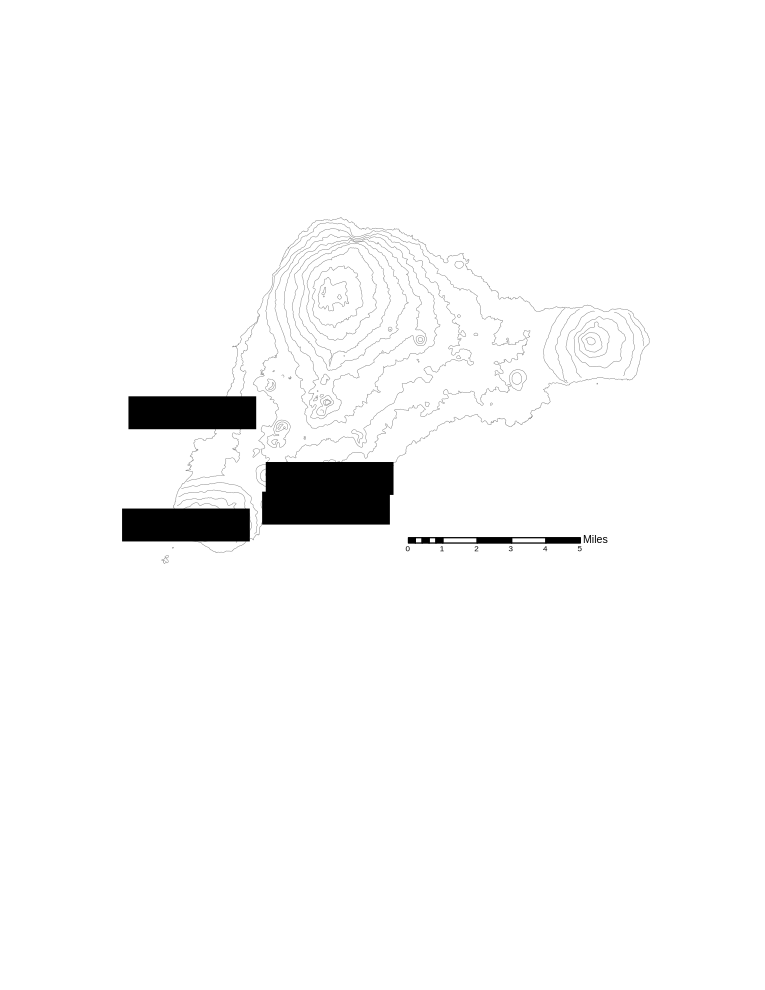
\includegraphics{../Figures/Figure2.pdf}

 Figure 3. \emph{Mata'a} included in the current analyses.

For the purposes of our analyses and following the approach taken in
Lipo et al. (2010), we assumed that \emph{mata'a} are the hafted
portions of compound tools that are otherwise incompletely preserved in
archaeological deposits. In this context and based on evidence of
usewear on the distal edges (Church \& Rigney 1994; Church \& Ellis
1996), we assume that the overall shape of \emph{mata'a} shape is a
functional element (sensu Dunnell 1978), the portion of the artifact
that interacts with the environment. Consequently, our interest is on
those aspects of shape that potentially affect function and thereby come
under natural selection. The task of explaining variability in shape
consists of identifying selective pressures that affect the performance
of shape and to determine whether their magnitude is sufficiently great
to impact fitness. The greater the selective pressures on performance,
the more constraint we would expect on those aspects of shape. If the
effect on function and performance is sufficiently small, then other
forces such as technological (i.e., material source, manufacturing
steps, etc.) or stylistic (stochastic or neutral) ones may have played a
role in fixing the shapes of \emph{mata'a}, as well as when and where
they occur in the archaeological record. In these cases, we would expect
to see a greater range of variability. It is possible, however, that not
all \emph{mata'a} instances were used in the same way. If \emph{mata'a}
shapes is influcenced by more than one function, either
contemporaneously or over time, then the selective context will differ
and thus the ``cause'' of \emph{mata'a} shape should vary. This
situation should create modal patterns of mata'a where shape variability
forms statistically distinguishablke groups.

\section{Data}\label{data}

In our analyses, we used scaled photos of \emph{mata'a} that we aligned
at the point where the midpoint of the stem meets the blade. We
converted the images to binary to isolate the artifact from the
background and then used TPSdig software (Rohlf 2014) to create outlines
of each \emph{mata'a}. TPSDig was particularly useful as it provides a
means for automatically tracing outlines with a fixed number of points.
In the creation of outlines, we identified 200 sets of X-Y coordinates
located on equidistant points along the perimeter of the artifact
(Figure 4). The set of coordinates for each mata'a were aggregated into
a single file using PAST (Hammer \emph{et al.} 2001).

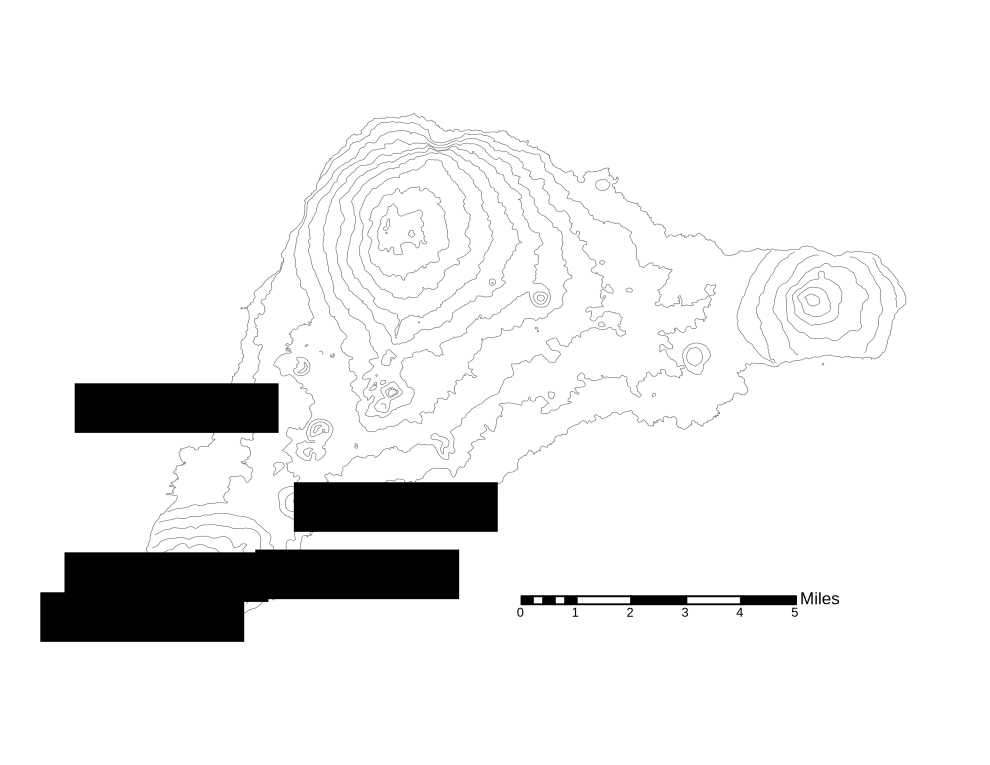
\includegraphics{../Figures/Figure3.jpg}

 Figure 5. \emph{Mata'a} length and width.

While the range of variability in shape shown in Figure 4 is
substantial, simple metrics of length and width (Figure 5) suggest that
there is just a single distribution of these objects without clear-cut
modes in size. Comparisons of length and width, however, are fairly
crude descriptions of shape. A more direct means of evaluating shape
variability is accomplished by superimposing \emph{mata'a} outlines
(Figure 6). This process required selecting a standard reference point
for all objects from which measurements would be based. We selected our
reference points, referred to here as ``centroids,'' based on the points
from which we believe variability will be meaningfully constrained (or
not). In this case of \emph{mata'a}, we chose a centroid at the center
of the haft where it intersects the blade.

 Figure 6. Superimposed \emph{mata'a} outlines from Rapa Nui. For
comparison, all \emph{mata'a} are aligned at the center point of the
haft where it meets the blade.

Once we identified the centroid, we calculated the distance from the
centroids to the perimeter in one-degree intervals for the 360-degree
perimeter. One-degree increments provide sufficient detail about shape
at a scale that characterized overall shape variability with enough
detail to capture attributes regarding the haft shape and distal blade
shape outline.\\While our measured outlines are composed of 200 points,
Momocs interpolates between points to locate distances from centroids at
even intervals.In addition, since all measurements are based on
georeferenced coordinates, planimetric measure (such as width or length)
can be calculated. Additional image analysis techniques to isolate
object outlines point to the strong potential for automation of the
measurement process, greatly increasing the ability to characterize
large assemblages. With large numbers of measures of radial distances
made relative to the \emph{mata'a} centroids, we then calculate a
statistical summary for each angle to assess variability in relative
dimensions (Figure 7).

 Figure 7. Variability in \emph{mata'a} shape shown with mean and 95\%
confidence intervals. Note that the 95\% confidence intervals are shown
with exaggerated differences between the values to areas with greater
variance versus those with more constrained shape.

\section{Morphometric Analyses}\label{morphometric-analyses}

Procrustes superimposition uses the the centroid of the shapes to (0,0)
as the bases for comparison between shapes. The centroid is calculated
on the based of average of the x and y coordinates. The shapes are then
scaled so that they are equivalent by multipling the coordinates of each
semilandmark by the suare root of the summed squared distances between
the centroid and each semilandmark. The algorithm then rotates each
shape until there is minimal distance between the shape and the mean
shape for all shapes. For the semilandmarks, the variation in position
of each semilandmark along the outline curve is also removed. Analyses
are done by projecting shapes onto a space tangent to shape space.
Within the tangent space, conventional multivariate statistical methods
such as multivariate analysis of variance and multivariate regression,
can be used to test statistical hypotheses about shape.

\begin{verbatim}
##  * No landmarks defined in $ldk, so trying to work on $coo directly.
## iteration:  1    gain: 598.82 
## iteration:  2    gain: 30.563 
## iteration:  3    gain: 5.5577 
## iteration:  4    gain: 0.35685 
## iteration:  5    gain: 4.6422 
## iteration:  6    gain: 1.3103 
## iteration:  7    gain: 0.75214 
## iteration:  8    gain: 0.059197 
## iteration:  9    gain: 0.49517 
## iteration:  10   gain: 0.29686 
## iteration:  11   gain: 0.059267 
## iteration:  12   gain: 0.00079621 
## iteration:  13   gain: 0.017054 
## iteration:  14   gain: 0.031944 
## iteration:  15   gain: 0.023498 
## iteration:  16   gain: 0.0017668 
## iteration:  17   gain: 0.011092 
## iteration:  18   gain: 0.011089 
## iteration:  19   gain: 0.005563 
## iteration:  20   gain: 0.00040004 
## iteration:  21   gain: 0.0023237 
## iteration:  22   gain: 0.0026083 
## iteration:  23   gain: 0.0014627 
## iteration:  24   gain: 0.00013552 
## iteration:  25   gain: 0.00060613 
## iteration:  26   gain: 0.00067535 
## iteration:  27   gain: 0.00037508 
## iteration:  28   gain: 3.9434e-05 
## iteration:  29   gain: 0.00014886 
## iteration:  30   gain: 0.00017024 
## iteration:  31   gain: 9.6677e-05 
## iteration:  32   gain: 1.1582e-05 
## iteration:  33   gain: 3.7073e-05 
## iteration:  34   gain: 4.3205e-05 
## iteration:  35   gain: 2.4881e-05 
## iteration:  36   gain: 3.322e-06 
## iteration:  37   gain: 9.1873e-06 
## iteration:  38   gain: 1.094e-05 
## iteration:  39   gain: 6.4025e-06 
## iteration:  40   gain: 9.4266e-07 
## iteration:  41   gain: 2.2763e-06 
## iteration:  42   gain: 2.7706e-06 
## iteration:  43   gain: 1.6469e-06 
## iteration:  44   gain: 2.6462e-07 
## iteration:  45   gain: 5.6312e-07 
## iteration:  46   gain: 7.013e-07 
## iteration:  47   gain: 4.2349e-07 
## iteration:  48   gain: 7.3665e-08 
## iteration:  49   gain: 1.3913e-07 
## iteration:  50   gain: 1.7745e-07 
## iteration:  51   gain: 1.0886e-07 
## iteration:  52   gain: 2.0358e-08 
## iteration:  53   gain: 3.4324e-08 
## iteration:  54   gain: 4.4882e-08 
## iteration:  55   gain: 2.7972e-08 
## iteration:  56   gain: 5.5916e-09 
## iteration:  57   gain: 8.4547e-09 
## iteration:  58   gain: 1.1347e-08 
## iteration:  59   gain: 7.185e-09 
## iteration:  60   gain: 1.528e-09 
## iteration:  61   gain: 2.0809e-09 
## iteration:  62   gain: 2.8667e-09 
## iteration:  63   gain: 1.8445e-09 
## iteration:  64   gain: 4.1473e-10 
## iteration:  65   gain: 5.0932e-10 
## iteration:  66   gain: 7.2396e-10 
## iteration:  67   gain: 4.7294e-10 
## iteration:  68   gain: 1.1278e-10 
## iteration:  69   gain: 1.2733e-10 
## iteration:  70   gain: 1.819e-10 
## iteration:  71   gain: 1.2005e-10 
## iteration:  72   gain: 3.2742e-11
\end{verbatim}

\subsection{By Source}\label{by-source}

\begin{Shaded}
\begin{Highlighting}[]
\CommentTok{#,fig.width=4.5,fig.height=4.5\}}

\KeywordTok{plot}\NormalTok{(}\KeywordTok{PCA}\NormalTok{(RapaF), }\StringTok{"Source"}\NormalTok{)}
\end{Highlighting}
\end{Shaded}

\begin{Shaded}
\begin{Highlighting}[]
\CommentTok{#, fig.width=4.5,fig.height=4.5\}}
\KeywordTok{plot}\NormalTok{(}\KeywordTok{PCA}\NormalTok{(RapaFP), }\StringTok{"Source"}\NormalTok{) }\CommentTok{# Procrustes aligned (normalization of the outlines)}
\end{Highlighting}
\end{Shaded}

\subsection{By Site}\label{by-site}

\begin{Shaded}
\begin{Highlighting}[]
\CommentTok{#, fig.width=4.5,fig.height=4.5\}}
\KeywordTok{plot}\NormalTok{(}\KeywordTok{PCA}\NormalTok{(RapaF), }\StringTok{"Site"}\NormalTok{) }\CommentTok{# regular EFT with normalized coefficients}
\end{Highlighting}
\end{Shaded}

\begin{Shaded}
\begin{Highlighting}[]
\CommentTok{#, fig.width=4.5,fig.height=4.5\}}
\KeywordTok{plot}\NormalTok{(}\KeywordTok{PCA}\NormalTok{(RapaFP), }\StringTok{"Site"}\NormalTok{) }\CommentTok{# Procrustes aligned (normalization of the outlines)}
\end{Highlighting}
\end{Shaded}

\section{Some embedded plots.}\label{some-embedded-plots.}

\begin{Shaded}
\begin{Highlighting}[]
\CommentTok{#, fig.width=4.5,fig.height=4.5\}}
\KeywordTok{plot}\NormalTok{(}\KeywordTok{PCA}\NormalTok{(RapaFP), }\StringTok{"Site"}\NormalTok{) }\CommentTok{# Procrustes aligned (normalization of the outlines)}
\end{Highlighting}
\end{Shaded}

\section*{References Cited}\label{references-cited}
\addcontentsline{toc}{section}{References Cited}

\textsc{Araho}, N. 1997. \emph{Obsidian stemmed tools from west new
britain, papua new guinea}. University of Sydney.

\textsc{Bahn}, P. \& J. \textsc{Flenley}. 1992. \emph{Easter island,
earth island}. London: Thames; Hudson.

\textsc{Balfour}, H. 1917. Some ethnological suggestions in regard to
easter island, or rapanui \emph{Folklore} 28: 356--81.

\textsc{Bollt}, R., J.E. \textsc{Clark}., P.R. \textsc{Fisher}. \& H.K.
\textsc{Yoshida}. 2006. An experiment in the replication and
classification of easter island mata'a \emph{Rapa nui journal} 20:
125--33.

\textsc{Bonhomme}, V. 2012. A graphical introduction to momocs and
outline analysis using r.
\url{http://www.vincentbonhomme.fr/Momocs/vignettes/}.

\textsc{Bonhomme}, V., S. \textsc{Picq}., C. \textsc{Gaucherel}. \& J.
\textsc{Claude}. 2014. Momocs: Outline analysis using r \emph{Journal of
Statistical Software} 56: 1--24.

\textsc{Bookstein}, F.L. 1982. Foundations of morphometrics \emph{Annual
Review of Ecology and Systematics}, 451--70.
\url{http://www.filogenetica.org/cursos/deluna/morfometria/referencias en pdf/Bookstein82.pdf}.

--- 1991. \emph{Morphometrics tools for landmarks data}. Cambridge
University Press.

--- 1997. Landmark methods for forms without landmarks: morphometrics of
group differences in outline shape \emph{Medical image analysis} 1:
225--43. \url{http://femininebeauty.info/i/bookstein.sliding.pdf}.

\textsc{Bookstein}, F.L., B. \textsc{Chernoff}., R.L. \textsc{Elder}.,
J. \textsc{Humphries}., G.R. \textsc{Smith}. \& R.E. \textsc{Strauss}.
1985. \emph{Morphometrics in evolutionary biology: the geometry of size
and shape change, with examples from fishes}. Academy of Natural
Sciences of Philadelphia Philadelphia.

\textsc{Bork}, H.-R., A. \textsc{Mieth}. \& B. \textsc{Tschochner}.
2004. Nothing but stones? A review of the extent and technical efforts
of prehistoric stone mulching on rapa nui \emph{Rapa nui journal} 18:
10--14.

\textsc{Bowman}, A. 2009. Review of 'morphometrics with r' \emph{Journal
of Statistical Software} 31: 1--2.

\textsc{Cardillo}, M. 2010. Some applications of geometric
morphometricsto archaeology, in A. Elewa (ed.) \emph{Morphometrics for
nonmorphometricians}: 325--41. Springer-Verlag.

\textsc{Church}, F. \& G. \textsc{Ellis}. 1996. A use-wear analysis of
obsidian tools from an ana kionga \emph{Rapa nui journal} 10: 81--88.

\textsc{Church}, F. \& J. \textsc{Rigney}. 1994. A microwear analysis of
tools from site 10-241, easter island--an inland processing site
\emph{Rapa nui journal} 8: 101--5.

\textsc{Claude}, J. 2008. \emph{Morphometrics with r}. Springer.

\textsc{Diamond}, J. 1995. Easter's end \emph{Discover} 9: 62--69.

--- 2005. \emph{Collapse: How societies choose to fail or succeed}. New
York: Viking.

\textsc{Dunnell}, R.C. 1978. Style and function: A fundamental dichotomy
\emph{American Antiquity} 43: 192--202.

--- 1986. Methodological issues in americanist artifact classification
\emph{Advances in archaeological method and theory} 9: 149--207.

\textsc{Edwards}, E., R. \textsc{Marchetti}., L. \textsc{Dominichetti}.
\& O. \textsc{Gonzales-Ferran}. 1996. When the earth trembled, the
statues fell \emph{Rapa nui journal} 10: 1--15.

\textsc{Flenley}, J. \& P.G. \textsc{Bahn}. 2003. \emph{The enigmas of
easter island: island on the edge}. Oxford ; New York: Oxford University
Press.

\textsc{Gunz}, P. \& P. \textsc{Mitteroecker}. 2013. Semilandmarks: a
method for quantifying curves and surfaces \emph{Hystrix, the Italian
Journal of Mammalogy} 24: 103--9.
\url{http://www.italian-journal-of-mammalogy.it/article/download/6292/pdf_6292}.

\textsc{Haedo}, F.G. de. \& J. \textsc{Roggeveen}. 1908. \emph{The
voyage of captain don felipe gonzález: In the ship of the line san
lorenzo, with the frigate santa rosalia in company, to easter island in
1770-1}. Vol. (13). 13. Hakluyt society.

\textsc{Hammer}, {Ø}., \textsc{Harper} D.A.T. \& \textsc{P. D. Ryan}.
2001. PAST: Paleontological statistics software package for education
and data analysis \emph{Palaeontologia Electronica} 4: 1--9.

\textsc{Heyerdahl}, T. 1989. \emph{Easter island--the mystery solved}.
London: Souvenir Press.

\textsc{Heyerdahl}, T. \& E. \textsc{Ferdon}. 1965. Reports of the
norwegian archaeological expedition to easter island and the east
pacific 2. London: Allen; Unwin.

\textsc{Hunt}, T.L. 2007. Rethinking easter island's ecological
catastrophe \emph{Journal of archaeological science} 34: 485--502.

\textsc{Hunt}, T.L. \& C.P. \textsc{Lipo}. 2006. Late colonization of
easter island \emph{Science} 311: 1603--6.
\url{\textless{}Go to ISI\textgreater{}://000236029500044}.

\textsc{Hunt}, T.L. \& C.P. \textsc{Lipo}. 2007. Chronology,
deforestation, and `collapse:' evidence vs. faith in rapa nui prehistory
\emph{Rapa nui journal} 21: 85--97.

--- 2009a. Revisiting rapa nui (easter island) `ecocide' \emph{Pacific
science} 63: 601--16.

--- 2009b. Ecological catastrophe, collapse, and the myth of `ecocide'on
rapa nui (easter island), in P.A. McAnany \& N. Yoffee (ed.)
\emph{Questioning collapse: Human resilience, ecological vulnerability,
and the aftermath of empire}: 21--44. New York: Cambridge University
Press.

--- 2011a. Easter island's complex history \emph{Nature} 479: 41.

\textsc{Hunt}, T.L. \& C.P. \textsc{Lipo}. 2011b. \emph{The statues that
walked}.

\textsc{Kendall}, D. 1989. A survey of the statistical theory of shape.
\emph{Statistical Science} 4: 8--120.

\textsc{Ladefoged}, T., C. \textsc{Stevenson}., P. \textsc{Vitousek}. \&
O. \textsc{Chadwick}. 2005. Soil nutrient depletion and the collapse of
rapa nui society \emph{Rapa nui journal} 19: 100--105.

\textsc{Ladefoged}, T.N., A. \textsc{Flaws}. \& C.M. \textsc{Stevenson}.
2013. The distribution of rock gardens on rapa nui (easter island) as
determined from satellite imagery \emph{Journal of archaeological
science} 40: 1203--12.
\url{http://ac.els-cdn.com/S0305440312004049/1-s2.0-S0305440312004049-main.pdf?_tid=f191146e-3120-11e3-a2fe-00000aab0f27\&acdnat=1381350511_fcbdd8c0c5fa27f7cfbeca2d9d9b645e}.

\textsc{Ladefoged}, T.N., C.M. \textsc{Stevenson}., S. \textsc{Haoa}.,
M. \textsc{Mulrooney}., C. \textsc{Puleston}., P.M. \textsc{Vitousek}.
\& O.A. \textsc{Chadwick}. 2010. Soil nutrient analysis of rapa nui
gardening \emph{Archaeology in oceania} 45: 80--85.
\url{http://oceania.metapress.com/index/TQ0202781J021860.pdf}.

\textsc{Lipo}, C.P. \& T.L. \textsc{Hunt}. 2009. AD 1680 and rapa nui
prehistory \emph{Asian perspectives} 48: 309--17.

\textsc{Lipo}, C.P. \& T.L. \textsc{Hunt}. 2014. Easter island,
archaeological evidence, and the evolutionary history of warfare
\emph{The 79th annual society for american archaeology meeting}. Austin,
TX: Society for American Archaeology.

\textsc{Lipo}, C.P., T.D. \textsc{Hunt}. \& R.C. \textsc{Dunnell}. 2012.
Formal analyses and functional accounts of groundstone `plummets' from
poverty point, louisiana \emph{Journal of archaeological science} 39:
84--91.
\url{http://www.sciencedirect.com/science/article/pii/S0305440311003220}.

\textsc{Lipo}, C.P., T.L. \textsc{Hunt}. \& S.R. \textsc{Haoa}. 2013.
The 'walking' megalithic statues (moai) of easter island \emph{Journal
of archaeological science} 40: 2859--66.
\url{http://ac.els-cdn.com/S0305440312004311/1-s2.0-S0305440312004311-main.pdf?_tid=f622ffde-26d9-11e3-8676-00000aab0f6b\&acdnat=1380220513_ddb22278741acb37f8d0b21c65e7d41a}.

\textsc{Lipo}, C.P., T.L. \textsc{Hunt}. \& B. \textsc{Hundtoft}. 2010.
Stylistic variability of stemmed obsidian tools (mata'a), frequency
seriation, and the scale of social interaction on rapa nui (easter
island) \emph{Journal of archaeological science} 37: 2551--61.
\url{http://www.sciencedirect.com/science/article/pii/S0305440310001779}.

\textsc{Metraux}, A. 1957. Easter island: A stone-age civilization of
the pacific.

\textsc{Mieth}, A., H. \textsc{Bork}., J. \textsc{McNeill}. \& V.
\textsc{Winiwarter}. 2010. The dynamics of soil, landscape and culture
on easter island (chile). \emph{Soils and societies: perspectives from
environmental history}, 273--321.
\url{http://www.cabdirect.org/abstracts/20103285130.html}.

\textsc{Morrison}, A. 2012. An archaeological analysis of rapa nui
settlement structure: A multi-scalar approach \emph{Department of
anthropology} Ph.D. University of Hawai'i, Manoa.

\textsc{Mulloy}, W. 1961. Ceremonial center of vinapu, in

\textsc{Mulrooney}, M. 2012. Continuity or collapse? Diachronic
settlement and land use in hanga ho`onu, rapa nui (easter island).
\emph{Department of anthropology} Ph.D. University of Auckland.

\textsc{Mulrooney}, M., T.N. \textsc{Ladefoged}., C.M.
\textsc{Stevenson}. \& S. \textsc{Haoa}. 2009. The myth of aD 1680: New
evidence from hanga ho'Onu, rapa nui (easter island) \emph{Rapa nui
journal} 23: 94--105.

\textsc{Mulrooney}, M.A., A. \textsc{McAlister}., C.M.
\textsc{Stevenson}., A.E. \textsc{Morrison}. \& L. \textsc{Gendreau}.
2014. Sourcing rapa nui mata`a from the collections of bishop museum
using non-destructive pXRF \emph{Journal of the Polynesian Society} In
Press.

\textsc{Rainbird}, P. 2002. A message for our future? The rapa nui
(easter island) ecodisaster and pacific island environments \emph{World
archaeology} 33: 436--51.
\url{http://links.jstor.org/sici?sici=0043-8243(200202)33\%3A3\%3C436\%3AAMFOFT\%3E2.0.CO\%3B2-W}.

\textsc{Rohlf}, F.J. 1990. Morphometrics. \emph{Annual Review of Ecology
and Systematics} 21: 299--316.

--- 2014. \url{http://life.bio.sunysb.edu/ee/rohlf/software.html}.

\textsc{Routledge}, K. 1919. The mystery of easter island: The story of
an expedition.

\textsc{Saher}, H. von. 1990. Some details from the journal of captain
bouman on the discovery of easter island \emph{Rapa nui journal} 6:
34--39.

\textsc{Skinner}, H.D. 1958. Some recent publications relating to easter
island culture and its probable history \emph{The journal of the
polynesian society} 67: 248--51.

\textsc{Specht}, J., R. \textsc{Fullagar}., R. \textsc{Torrence}. \& N.
\textsc{Baker}. 1988. Prehistoric obsidian exchange on melanesia: A
perspective from the talasea sources \emph{Australian Archaeology},
3--16. \url{http://www.jstor.org/stable/40286657}.

\textsc{Stevenson}, C.M., T.L. \textsc{Jackson}., A. \textsc{Mieth}.,
H.-R. \textsc{Bork}. \& T.N. \textsc{Ladefoged}. 2006. Prehistoric and
early historic agriculture at maunga orito, easter island (rapa nui),
chile \emph{Antiquity} 80: 919--36.

\textsc{Stevenson}, T.L., C. M. \& S. \textsc{Haoa}. 2002. Agricultural
production in an uncertain environment \emph{Rapa nui journal} 16.

\textsc{Thompson}, D.W. 1917. \emph{On growth and form}. Cambridge
University Press.

\textsc{Torrence}, R., S. \textsc{Kelloway}. \& P. \textsc{White}. 2013.
Stemmed tools, social interaction, and voyaging in early--mid holocene
papua new guinea \emph{The Journal of Island and Coastal Archaeology} 8:
278--310.
\url{http://www.tandfonline.com/doi/abs/10.1080/15564894.2012.761300}.

\textsc{Torrence}, R., P. \textsc{Swadling}., W. \textsc{Ambrose}., N.
\textsc{Kononenko}., P. \textsc{Rath}. \& M. \textsc{Glascock}. 2009.
Obsidian stemmed tools and mid-holocene interaction \emph{Asian
Perspectives} 48: 118--47.

\textsc{Torrence}, R., P. \textsc{Swadling}., N. \textsc{Kononenko}., W.
\textsc{Ambrose}., P. \textsc{Rath}. \& M.D. \textsc{Glascock}. 2009.
Mid-holocene social interaction in melanesia: New evidence from
hammer-dressed obsidian stemmed tools \emph{Asian Perspectives} 48:
119--48.
\url{http://scholarspace.manoa.hawaii.edu/bitstream/handle/10125/29084/AP_V48No1_torrence.pdf?sequence=1}.

\textsc{Wilmshurst}, J.M., T.L. \textsc{Hunt}., C.P. \textsc{Lipo}. \&
A. \textsc{Anderson}. 2011. High-precision radiocarbon dating shows
recent and rapid initial human colonization of east polynesia
\emph{Proceedings of the national academy of science} 108: 1815--20.

\end{document}
